\section{ Di-Higgs Analysis }
\fullscreenimage{VBF Di-Higgs Analysis}{vbf-hh_diagrams}
\frame{
    \frametitle{ VBF $\rightarrow$ HH $\rightarrow$ $\fourB$ }

    \begin{columns}
        \begin{column}{0.5\textwidth}
            { \small
                I've joined the VBF to 4b dihiggs subgroup, to look into improving selection of VBF jets in the final state.
                Ultimate goal would be putting a better limit on the $C_{2V}$ coupling constant.
            }

            \begin{figure}
                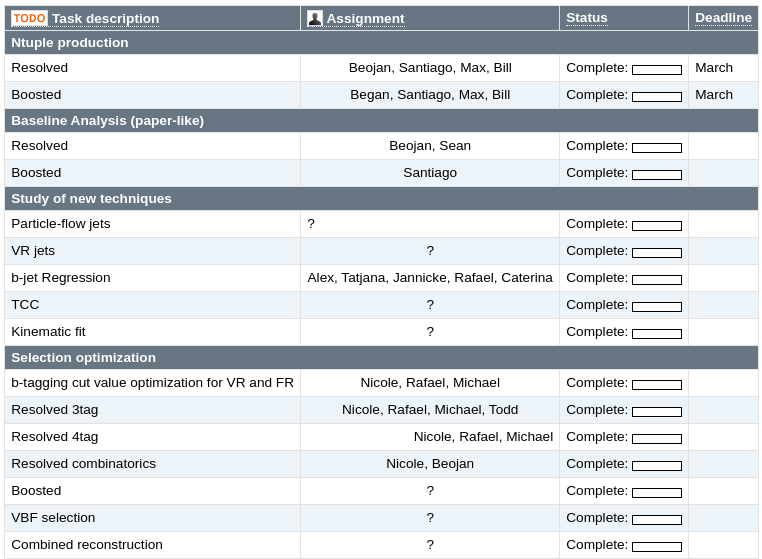
\includegraphics[width=\linewidth,height=\textheight,keepaspectratio]
                {dihiggs_task_list}
            \end{figure}
        \end{column}
        \begin{column}{0.5\textwidth}
            \resizebox{0.50\textheight}{!}{
                \resizebox{.8\textwidth}{!}{
\begin{tikzpicture} \begin{feynman}
    \vertex (c2v) {???};
    \vertex [above right=of c2v] (h1) {$h_1$};
    \vertex [below right=of c2v] (h2) {$h_2$};
    \vertex [above left=of c2v] (vb1);
    \vertex [below left=of c2v] (vb2);
    \vertex [left=of vb1] (q1) {$q_1$};
    \vertex [left=of vb2] (q2) {$q_2$};
    \vertex [above right=of h1] (b1) {$b$};
    \vertex [below right=of h2] (bbar2) {$\bar b$};
    \vertex [below=of b1] (bbar1) {$\bar b$};
    \vertex [above=of bbar2] (b2) {$b$};

    \vertex [above=of b1] (q3) {$q_3$};
    \vertex [below=of bbar2] (q4) {$q_4$};

    \diagram* {
        (q1) -- (vb1) -- (q3),
        (q2) -- (vb2) -- (q4), 
        (vb1) -- [boson] (c2v) -- [boson] (vb2),
        (h1) -- [scalar] (c2v) -- [scalar] (h2),
        (b1) -- (h1) -- (bbar1),
        (b2) -- (h2) -- (bbar2),
    };
\end{feynman} \end{tikzpicture}
}

            }
        \end{column}
    \end{columns}
}


% Initial Task: how often are the higgs pairs/vbf pairs correctly identified?
% Current approach is a BDT to identify the two jet pairs that correspond to the higgss,
% and then use a number of heuristic cuts to choose vbf jets* (I think...)
% Using ML and jet substructure tools, can I do better?
